\documentclass[times, utf8, diplomski]{fer}
\usepackage{booktabs}
\usepackage[final]{pdfpages}

\begin{document}

% TODO: Navedite broj rada.
\thesisnumber{1719}

% TODO: Navedite naslov rada.
\title{Razvoj sustava globalne vizije za testiranje algoritama upravljanja bespilotnim letjelicama}

% TODO: Navedite vaše ime i prezime.
\author{Bojan Spahija}

\maketitle

% Ispis stranice s napomenom o umetanju izvornika rada. Uklonite naredbu \izvornik ako želite izbaciti tu stranicu.
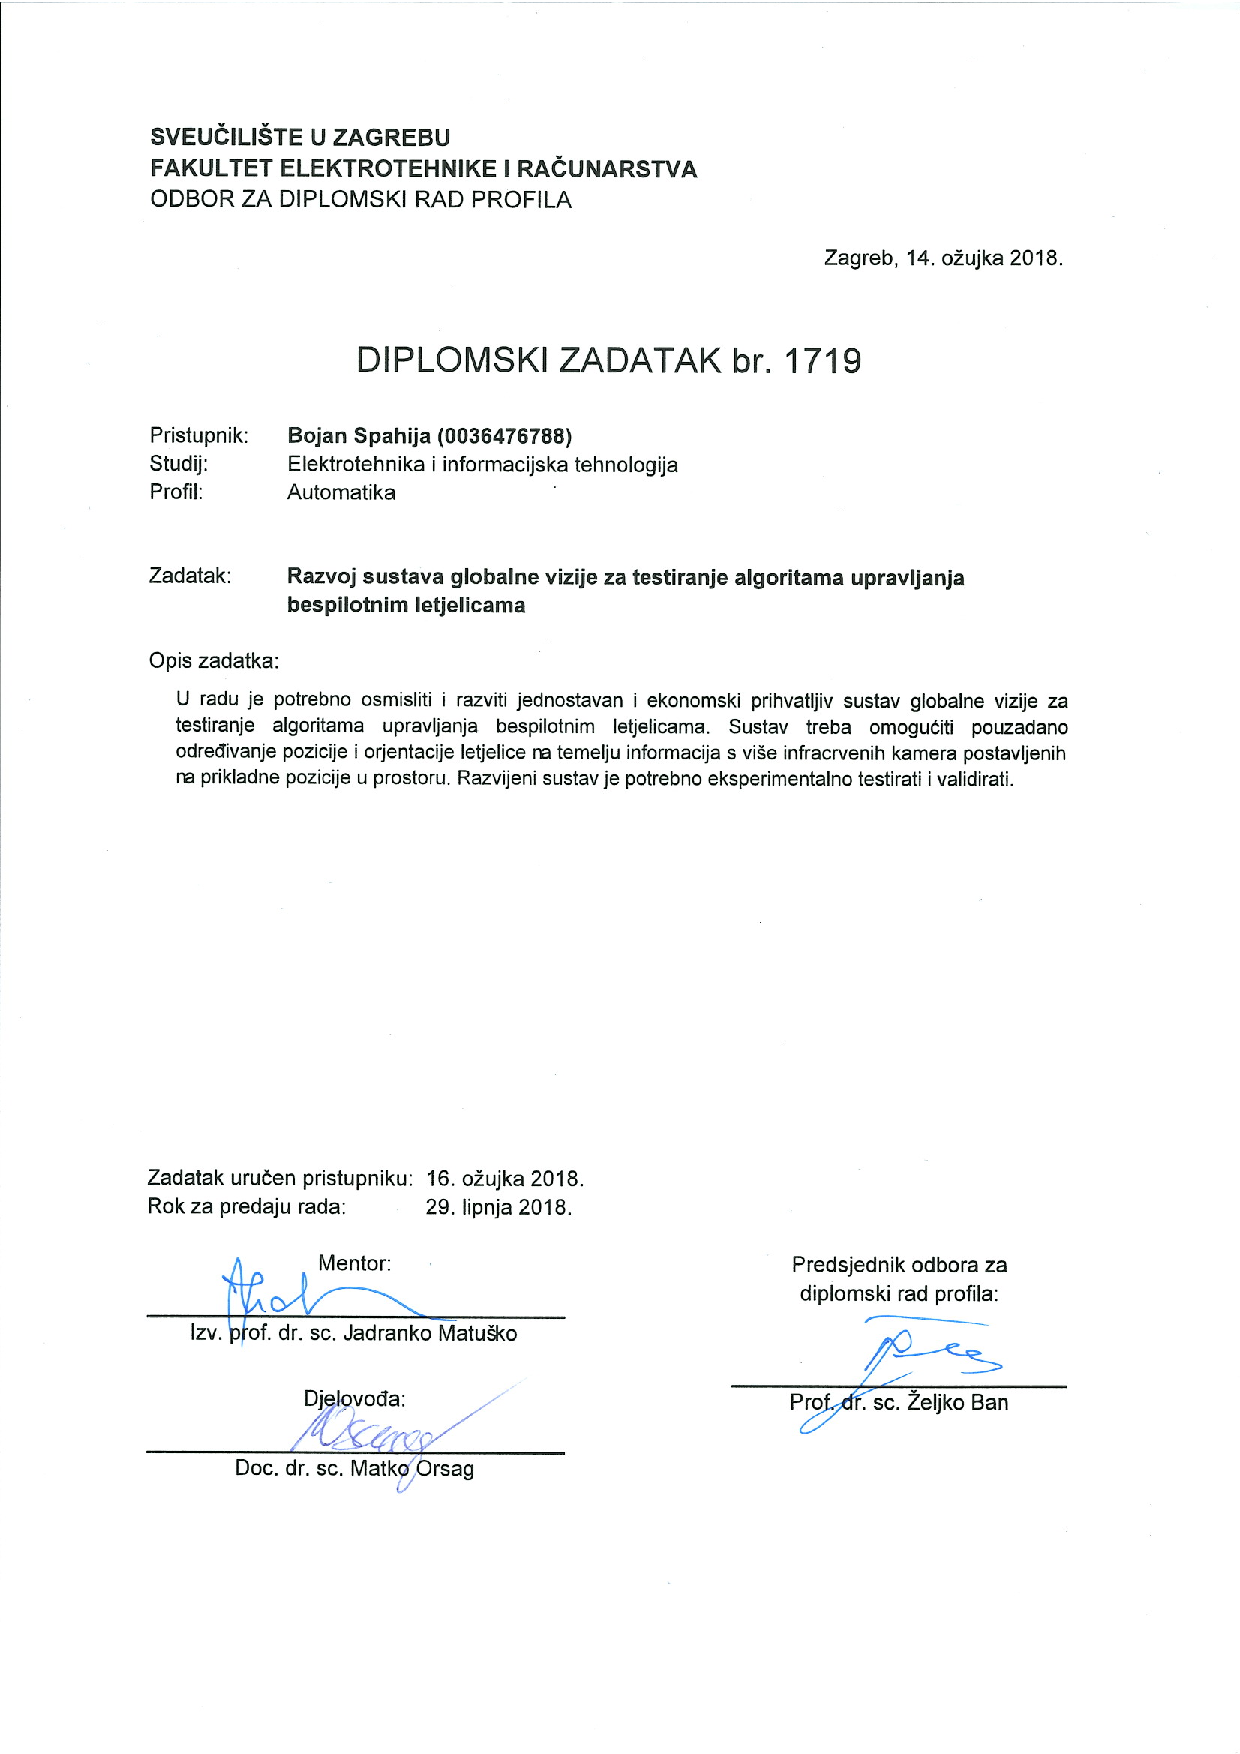
\includepdf[pages=-]{img/izvornik.pdf}

% Dodavanje zahvale ili prazne stranice. Ako ne želite dodati zahvalu, naredbu ostavite radi prazne stranice.
\zahvala{Svim ljudima dobre volje}

\tableofcontents

\listoffigures

\chapter{Uvod}
U mnogim granama industrije veliki značaj ima praćenje kretanja. Praćenje pokreta koristi se kod animacija za filmsku industriju i industriju video igara. Koristi se u vojnoj industriji za simulatore i u znanstvene svrhe za proučavanje kretanja ljudi i životinja. Zbog napretka robotike u posljednjih nekoliko godina, sve je veća potreba za preciznim praćenjem dronova i drugih robota s ciljem poboljšanja i razvoja algoritama autonomnog upravljanja.

Trenutna rješenja praćenja pokreta poput OptiTrack-a omogućuju iznimno precizno praćenje, ali vrlo su skupa. Cijene se kreću od nekoliko tisuća dolara do nekoliko desetaka tisuća dolara što nije prikladno za male firme, pojedince ili projekte za koje nije potrebna tolika preciznost. 

\chapter{Postav}
Za 3D lokalizaciju bespilotne letjelice potrebne su minimalno dvije kamere. Pomoću dvije kamere i markera koje te kamere mogu detektirati moguće je dobiti lokaciju tog markera odnosno x-y-z koordinate markera u globalnom koordinatnom sustavu. Kod upravljanja letjelicom važno je poznavati i orijentaciju letjelice (yaw). 

Upravljačke vrijednosti koje šaljemo letjelici imaju direktan utjecaj na gibanje letjelice u njezinom lokalnom koordinatnom sustavu. Da bi se poznavao utjecaj upravljačkih vrijednosti na gibanje u globalnom koordinatnom sustavu, potrebno je znati za koliko je zarotiran lokalni koordinatni sustav letjelice u odnosu na globalni koordinatni sustav (orijentacija). Kako bismo dobili informaciju o orijentaciji, potreban je specifični raspored markera koji nam omogućuje prepoznavanje orijentacije bez poznavanja orijentacije u prethodnim trenucima.

\section{Izbor kamera, IC izvora i markera}
Sustav globalne vizije mora zadovoljiti određene zahtjeve i uvjete:
\begin{itemize}
	\item Detekcija će se odvijati u zatvorenom prostoru
	\item Maksimalna udaljenost markera od kamere je oko 4m
	\item Letjelica je malih dimenzija što limitira dimenziju markera 
\end{itemize}
Zbog relativno velike udaljenosti na kojoj detekcija markera mora raditi i malih dimenzija markera, detekcija pomoću RGB kamera i markera u bojama nije pouzdana. U sustavu globalne vizije koristit će se detekcija pomoću infracrvene svijetlosti.

Infracrvena svjetlost je pogodna za detekciju na većim udaljenostima i uvjetima promjenjivog osvjetljenja. Većina materijala iz okoline reflektira vrlo malo infracrvene svjetlosti što osigurava pouzdanu detekciju infracrvenih izvora i materijala koji dobro reflektiraju infracrvenu svjetlost. Za detekciju pomoću infracrvene svjetlosti potrebni su okrugli markeri koji dobro reflektiraju infracrvenu svjetlost u svim smjerovima, kamere koje će detektirati svjetlost reflektiranu od markera i izvor infracrvene svjetlosti dovoljno velikog intenziteta i kuta zračenja da pokrije cijelo vidno polje kamere i željenu maksimalnu udaljenost markera.

\subsection{Kamera}
Testirane kamere su bile Pixy kamera sa IR-LOCK infracrvenom lećom i kamera unutar Wiimotea koja ima već infracrvenu leću. Obje kamere vraćaju piksele slike na kojima je detektirano infracrveno zraćenje. Valna duljina infracrvenog zraćenja koje kamere najbolje detektiraju iznosi oko 940nm. Wiimote šalje piksele od 4 najintenzivije infracrvene točke dok ih Pixy kamera može detektirati mnogo više, što u ovom slučaju ne igra ulogu zbog samo 3 potrebne točke.

Veza između Wiimotea i računala postiže se Bluetooth povezivanjem. Takva veza omogućuje veću udaljenost kamera i veću fleksibilnost kod postavljanja kamera. Direktna veza između računala i Pixy kamere može se postići mini USB kablom, a ako je nužna bežična veza potrebno je spojiti Pixy kameru na mikrokontroler koji će onda komunicirati bežično s računalom.

Također je važan vidni kut kamere jer on određuje veličinu prostora koji će se moći nadzirati. Kod Wiimote kamere horizontalni vidni kut iznosi oko 42$^{\circ}$, dok vertikalni vidni kut iznosi oko 32$^{\circ}$. Pixy kamera pokriva veće područje s horizontalnim vidnim kutem od 75$^{\circ}$ i vertikalnim vidnim kutem od 47$^{\circ}$. U segmentu vidnog polja Pixy kamera ima prednost.

Rezolucija kamere će utjecati na preciznost izračuna 3D globalnih koordinata točke. Niže rezolucije rezultiraju većim pogreškama određivanja pozicije objekata u daljini. Wiimote kamera ima vrlo malu rezoluciju od 128x96. Procesor unutar Wiimotea povećava tu rezoluciju na 1024x768 pomoću postupka analize intenziteta rubnih piksela i izračuna pozicije infracrvene točke unutar piksela (8x subpixel analysis). Ovaj postupak povećanja rezolucije kamere uvelike poboljšava preciznost detekcije usprkos korištenju jeftinih komponenata (infracrvena kamera niske rezolucije i mikroprocesor).\\
S druge strane, Pixy kamera ima ugrađenu mnogo kvalitetniju Omnivision OV9715 kameru veće rezolucije (1280x800). Pri takvoj rezoluciji, Pixy kamera radi na 25 sličica u sekundi. Kako bi se postigla veća brzina rada kamere (50 sličica u sekundi), smanjena je rezolucija na 640x400. Zbog ograničenja RAM-a koji Pixy koristi za obradu slike, rezolucija je dodatno smanjena na 320x200 piksela. Veća rezolucija Wiimotea ga čini boljim izborom zbog manje greške detekcije, a i manje cjene. Wiimote je moguće nabaviti po cijeni nižoj od \$20, dok Pixy kamera košta \$69.99.

Wiimote je bolji izbor zbog rezolucije, lakšeg povezivanja i postavljanja te niže cijene. Jedina mana mu je relativno usko vidno polje, ali taj problem se može riješiti dobrim pozicioniranjem kamera na dovoljnu udaljenost od radnog područja drona.

\subsection{Infracrveni LED izvor}
Potrebno je montirati izvor infracrvene svjetlosti uz kameru i usmjeriti ga u smjeru gledanja kamere kako bi se dobila čim bolja detekcija markera. Izvor mora biti dovoljnog intenziteta da infracrvena svjetlost bude detektirana kamerom nakon što prođe udaljenost između kamere i markera, reflektira se od markera i vrati opet do kamere. U najudaljenijoj točci radnog prostora drona ta će udaljenost biti oko 4m. Obične jeftine infracrvene diode male snage takvu udaljenost neće moći uspješno pokriti za detekciju. Dodatni problem s takvim infracrvenim diodama je relativno mali kut zračenja koji iznosi najčešće između 15$^{\circ}$ i 30$^{\circ}$. Da bi se pokrio cijeli radni prostor drona i vidno polje kamere potrebno bi bilo staviti više takvih dioda oko kamere.

Kako bi cijeli radni prostor bio dobro osvijetljen, koristiti će se infracrveni LED čipovi visoke snage od 3W (SMD LED Module) koji generira svjetlost valne duljine od 940nm. Osim veće udaljenosti koju pokriva, prednost ovakve vrste LED izvora je u širokom kutu zračenja koji iznosi 120$^{\circ}$. Tijekom testiranja ispostavilo se da 3W infracrveni LED izvori u kombinaciji s reflektirajućim markerom omogućuju detekciju markera na premaloj udaljenosti od oko 1m. Da bi se ostvarila detekcija pomoću reflektirajućeg markera potrebno bi bilo koristiti izvor jači od 10W. Zbog širokog kuta zraćenja i visoke snage, LED izvori mogu se dobro detektirati na udaljenosti do 3m pa su pogodni za markere ako se montiraju na drona.

\subsection{Marker}
Markeri koji će se nalaziti na bespilotnoj letjelici moraju biti što lakši zbog iznimno male nosivosti letjelice. Drugi zahtjev je da reflektiraju što više svjetlosti natrag prema kameri neovisno o položaju letjelice i markera. Materijali koji dobro reflektiraju infracrvenu svjetlost su neki metali (Al, Ag i Au) te oksidi metala poput SiO$_2$ i Al$_2$O$_3$. Ukoliko bi se koristili premazi ili boje koje sadrže navedene spojeve i elemente, oni bi se trebali nanjeti na lagani materijal oblika kugle koji će reflektirati svjetlost natrag kameri. U ovom slučaju važno je da marker ima oblik kugle kako bi se dio reflektirane svjetlosti, neovisno o poziciji markera i kamere, uvijek vraćao istim putem natrag prema kameri. Stiroporne kuglice zadovoljavaju zahtjeve za marker koji će biti premazan.

Druga opcija je korištenje retroreflektirajućih materijala. Retroreflektirajući materijali reflektiraju svjetlost natrag izvoru svjetlosti uz minimalno rasipanje. Zraka svjetlosti koja dolazi prema retroreflektoru je paralelna i suprotnog smjera od reflektirane zrake. Retroreflektori su najčešće male staklene ili plastične prizme. Koriste se u prometu u boji za linije na cesti i prometne znakove, kod reflektirajućih prsluka,  očiju za bicikl, itd. U slučaju odabira retroreflektora nije nužno koristiti marker oblika kugle zbog svojstva da vraća svjetlost prema izvoru neovisno o kutu upada.

Zbog infracrvenog izvora premalog intenziteta nije moguće koristiti reflektirajuće markere pa će se sam izvor koristiti kao marker. Tri izvora pričvršćena su na bespilotnu letjelicu i spojena su u paraleli na dronovu bateriju. Ovim se zadovoljavaju uvjeti detekcije, ali se skraćuje trajanje baterije zbog dodatnog napajanja LED izvora. 

\section{Pozicija kamera i markera}
Za preciznu i robusnu detekciju važno je pozicionirati kamere i markere tako da u svakom mogućem stanju letjelice unutar radnog prostora markeri budu detektirani. Robusnost je moguće postići postavljanjem viška kamera kako bi u svakom slučaju barem tri kamere vidjele markere. Također je opcija ograničenje radnog prostora letjelice tako da smo sigurni da u svim pozicijama sve kamere vide markere. 

Koriste se tri markera pozicionirana na vrhu letjelice. Markeri su postavljeni u formaciju trokuta sa jednim markerom ispred prednjeg kraja letjelice dok su druga dva markera iza stražnjeg kraja letjelice. Razmak između stražnjih markera je manji od razmaka između stražnjih i prednjeg kako bi se detektirala orijentacija letjelice.

Obje kamere moraju detektirati sva tri markera da bi se mogla odrediti pozicija i orijentacija letjelice u globalnom koordinatnom sustavu. Kamere su postavljene na pano visine 1.88m i širine 1.25m. Pozicionirane su na rubovima panoa kako bi bile što udaljenije i pokrivale što veći radni prostor. Nagib kamera u odnosu na okomicu iznosi 42$^{\circ}$. Iz poznavanja maksimalne udaljenosti detekcije koja iznosi 3m te horizontalnog i vertikalnog vidnog kuta Wiimote kamera izračunava se područje unutar kojeg će obje kamere detektirati sva tri LED markera.

\subsection{Nosač za Wiimote}
Potrebno je napraviti nosač za Wiimote kamere kako bi se dobila precizna orijentacija kamera i čvrsta veza sa objektom na kojem će kamera biti postavljena (pano). Nosač za kameru mora imati mogućnost zakreta kamere oko dvije osi, osi x i y (gore-dolje, lijevo-desno). Iz izmjerenih dimenzija Wiimotea i segmenta panoa na koji će se nosač pričvrstiti, napravljen je model modularnog nosač u Solidworksu i isprintan pomoću 3D printera. Nosač se sastoji od 3 dijela:

\begin{enumerate}
	\item Držač Wiimotea
	\item Učvršćivač za pano
	\item Segment za vezu između fiksiranih dijelova 
\end{enumerate}

Veza između držača Wiimotea i segmenta za vezu ostvarena je preko ploha koje sjedaju jedne između drugih. Dok su plohe poravnate još postoji mjesta za micanje pa je moguće postaviti željenu rotaciju Wiimotea oko x-osi (gore-dolje). Kada je postavljeni željeni kut rotacije, umetanjem M3 vijka kroz rupu u plohama i njegovim zatezanjem pomoću matice učvršćuje se veza i osigurava željena rotacija.

Veza između dijela učvršćenog na pano i segmenta za povezivanje ostvarena je preko cilindra na koji se postavlja segment za povezivanje. Segment za povezivanje se može slobodno rotirati oko vertikalne osi (lijevo-desno). Kad se postavi željeni zakret Wiimotea, veza se učvršćuje pomoću M3 matice i vijka. 

\subsection{Radni prostor}
Iz pozicija i orijentacija kamera, poznatog vidnog kuta i maksimalne udaljenosti na kojoj Wiimoteovi detektiraju infracrveni LED marker računa se prostor unutar kojeg je kamera u mogućnosti detektirati marker. Taj postupak se radi za obje kamere. Presjek prostora detekcije prve i druge kamere je radni prostor. Ako dron ostane unutar tog prostora njegova pozicija i orijentacija će biti dobivene iz sustava globalne vizije pa je važno postaviti ograničenja radnog prostora u algoritme upravljanja dronom kako on ne bi izašao tog prostora.  

\chapter{Izračun pozicije i orijentacije}


\chapter{Komunikacija}

\chapter{Upravljanje}

\chapter{Zaključak}
Zaključak.

\bibliography{literatura}
\bibliographystyle{fer}

\begin{sazetak}
U mnogim granama industrije veliki značaj ima praćenje kretanja. Prisutna rješenja poput OptiTrack-a osiguravaju precizno praćenje, ali su iznimno skupa. Cilj rada je razvoj jednostavnog i ekonomski prihvatljivog sustava globalne vizije za praćenje pozicije i orijentacije bespilotnih letjelica. Sustav se sastoji od dvije infracrvene kamere i tri infracrvena markera postavljena na dronu. Za određivanje pozicije markera u globalnom koordinatnom sustavu potrebne su minimalno dvije kamere. Minimalno tri markera potrebna su kako bi se mogla izračunati orijentacija drona uz njegovu poziciju. Kao kamera se koristi Wiimote koji sadrži jednostavnu infracrvenu kameru, a markeri su infracrveni LED izvori velike snage (3W). Komunikacija između Wiimoteova i osobnog računala ostvarena je pomoću Bluetootha i ROS čvora. Iz poznatih pozicija kamera i dobivenih točaka od svakog Wiimotea, osobno računalo računa globalnu poziciju svake točke te iz tih pozicija računa orijentaciju i poziciju drona. Orijentacija i pozicija se objavljuju preko ROS-a kako bi se mogli dohvatiti od strane upravljačkog algoritma. 

\kljucnerijeci{praćenje pokreta, sustav vizije, dronovi, infracrvene kamere, Wiimote, markeri, pozicija, orijentacija, ROS}
\end{sazetak}
\newpage

% TODO: Navedite naslov na engleskom jeziku.
\engtitle{Development of a Global Vision System for Testing of Control Systems for Unmanned Aerial Vehicles}
\begin{abstract}
Motion tracking systems are of great importance in many industries. Current solutions like OptiTrack ensure precise tracking, but are very expensive. The goal of the project is the development of a simple and economically acceptable global vision system for drone position and orientation tracking. The system is made of two static infrared cameras and three infrared markers placed on the drone. To determine the position of the markers in the global coordinate system a minimum of two cameras is needed. At least three markers are needed in order to calculate the orientation of the drone. The camera used in the project is the IR camera inside a Wiimote and the markers used are high power IR LED sources (3W). The communication between the Wiimotes and the PC is realized using Bluetooth and a ROS node for each Wiimote. From the known Wiimote positions and the points detected by the Wiimotes, the PC calculates the global position of each point and then uses those positions to calculate the orientation and position of the drone. Orientation and position are published to a ROS topic, so that the control algorithm can acquire them.

\keywords{motion tracking, vision system, drones, infrared cameras, Wiimote, markers, position, orientation, ROS}
\end{abstract}

\end{document}
